%---------------------------------------------------------------------------------
\chapter{Implementation}
\label{chap:code-implementation}
%---------------------------------------------------------------------------------
\section{Software details}
The numerical methods implemented in this software are classified into three classes: one-step methods, predictor-corrector methods and adaptive methods. The methods included are:
\begin{enumerate}
    \item One-step method
    \begin{itemize}
        \item Euler's explicit method
        \item Euler's implicit method
        \item Trapezium rule method
        \item Four-stage Runge-Kutta method
    \end{itemize}
    \item Predictor-corrector method
    \begin{itemize}
        \item Euler-Trapezoidal method
    \end{itemize}
    \item Adaptive method
    \begin{itemize}
        \item BS23 algorithm
        \item RKF45 algorithm
    \end{itemize}
\end{enumerate}
The code is available on Github via \href{https://github.com/FarmHJ/numerical-solver}{this link}. There are badges displayed on the main page of the Github repository to indicate that the code are tested to work on several python versions and operating systems. One of the badges shows the code coverage of the software, which will be described in details in the next section \ref{sec:testing}. Finally, there is a status badge to verify that the documentation of the software is built successfully. The documentation of the software can be found \href{https://numerical-solver.readthedocs.io/en/latest/index.html}{here}.

\begin{figure}
    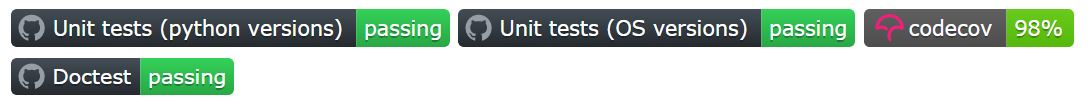
\includegraphics[width=0.95\columnwidth]{badges}
    \caption{Badges on Github repository}
    \label{fig:badges}
 \end{figure}

\section{Unit testing}
\label{sec:testing}
In the progress of constructing the software, a unit testing infrastructure was put in place. The purpose of the unit testing is to create a robust and sustainable software. Written codes are tested to make sure it runs as intended and reproduces expected results. If code is tested while writing, it would be easier to fix bugs in the future. 

Code coverage is used to define the percentage of codes covered in the unit testing process. It is usually aim to achieve a 100\% code coverage. However, a 100\% code coverage does not necessarily mean that the code is correct or free of errors. Nevertheless, it provides some confidence that the code is implemented correctly.

Every method in this numerical-solver software is tested, including the initialisation of the problem. The numerical solution produced by each method is tested to give the same solution as a manually calculated solution. The methods are mostly tested against the example model \ref{eqn:example_model}.

\section{Testing initialisation of problem}
The initialisations of each class are tested to ensure that variables are initialised correctly and input type satisfies the requirements. For example, 

\begin{lstlisting}[language=Python]
def test__init__(self):

    def func(x, y):
        return [-y[0]]
    x_min = 0
    x_max = 1
    initial_value = [1]
    mesh_points = 10

    problem = solver.OneStepMethods(
        func, x_min, x_max, initial_value, mesh_points)

    # Test initialisation
    self.assertEqual(problem.x_min, 0)
    self.assertEqual(problem.mesh_points, 10)

    # Test raised error for callable function
    with self.assertRaises(TypeError):
        solver.OneStepMethods(
            x_min, x_min, x_max, initial_value, mesh_points)

    # Test raised error if initial_value not list
    with self.assertRaises(TypeError):
        solver.OneStepMethods(
            func, x_min, x_max, 1, mesh_points)
\end{lstlisting}
. A simple model with known solution is first initialised. Required inputs were check to make sure the problem is set up properly, in line 14 and 15 of the code snippet above. To ensure that the inputs to the function are of the desired data type, errors are raised whenever the user inputs a wrong data type. The unit testing also tests that these errors are raised appropriately (line 17 to 25) whenever the data type does not satisfy the requirements. 

\section{Testing function}
After making sure the problem is properly initialised, we then test that the numerical methods are working correctly. Take the adaptive method, BS23 algorithm, as an example, 
\begin{lstlisting}[language=Python]
def test_ode23(self):

def func(x, y):
    return [-y[0]]
x_min = 0
x_max = 1
initial_value = [1]

problem = solver.AdaptiveMethod(
    func, x_min, x_max, initial_value, initial_mesh=0.5)
mesh, soln = problem.ode23()

# Test end point of mesh
self.assertGreaterEqual(mesh[-1], 1.0)

# Test mesh point
self.assertAlmostEqual(mesh[1], 0.3483788976565)

# Test solution at first stepsize
self.assertAlmostEqual(soln[1][0], 0.7052580305097)
\end{lstlisting}
The method is first tested to execute computations up to the maximum mesh point indicated. Then, it is checked that the first adaptive mesh point and its solution, obtained from the software, matches the value computed manually. 